% !TEX options = --shell-escape
% !TEX program = xelatex
\documentclass[]{USTBReport}

\USTBset{
    Course      = 计算机组成原理,  % 实验名称
    Instructor  = ,          % 指导老师
    Location    = ,   % 实验地点
    School      = 计通学院,        % 学院
    Score       = 100,        % 专业
    Class       = 计215,        % 班级
    Name        = 王雨辰,            % 姓名
    Number      = U202141xxx,        % 学号
    Year        = \the\year,       % 年
    Month       = \the\month,      % 月
    Day         = \the\day,        % 日
}
\usepackage{xeCJK}
\usepackage{booktabs}
\usepackage{longtable}
\usepackage{listings}
\usepackage{multirow}
\usepackage{multicol}
\usepackage{cleveref}
\usepackage{bookmark}
\usepackage{tabularx}
\usepackage{placeins}

\newcommand{\hl}[1]{\textbf{\textcolor{blue}{#1}}}

\lstset{
    language=Verilog,
    backgroundcolor = \color{cyan!10},    % 背景色:淡黄
    basicstyle = \small\ttfamily,           % 基本样式 + 小号字体
    rulesepcolor= \color{gray},             % 代码块边框颜色
    breaklines = true,                  % 代码过长则换行
    numbers = left,                     % 行号在左侧显示
    numberstyle = \small,               % 行号字体
    keywordstyle = \color{blue},            % 关键字颜色
    commentstyle =\color{purple!100},        % 注释颜色
    stringstyle = \color{red!100},          % 字符串颜色
    frame = shadowbox,                  % 用(带影子效果)方框框住代码块
    showspaces = false,                 % 不显示空格
    columns = fixed,                    % 字间距固定
    morekeywords = {as},                % 自加新的关键字(必须前后都是空格)
    deletendkeywords = {compile}        % 删除内定关键字;删除错误标记的关键字用deletekeywords删!
}
\begin{document}
%\makecover
    \maketitle


    \section{实验名称}
    单周期CPU指令扩展与仿真


    \section{实验要求}
    用VerilogHDL或VHDL语言在原处理器基础上扩展一条指令(现场给出),
    给出设计思路及扩展后的控制信号表格,仿真波形图,和对仿真波形的具体分析。
    最后提交该工程文件全部代码。代码应有适当的注释,并在实验报告中体现;
    报告中需要有指令的\hl{分析设计过程}(一定包括对\hl{数据通路}的分析),
    仿真验证过程需要有CPU运行的程序文件(带注释)、仿真波形图及\hl{波形分析}。

    \FloatBarrier
    \section{实验仪器}
    \begin{enumerate}
        \item OS: Win11 64位
        \item Software: Vivado2018.3开发工具
    \end{enumerate}


    \FloatBarrier
    \section{实验内容与步骤}

    \subsection{需要扩展的指令是:\texttt{XXX}}
    指令格式及功能说明:

    \subsection{指令执行过程分析(结合顶层数据通路图分析)}
    \begin{figure}
        \centering
        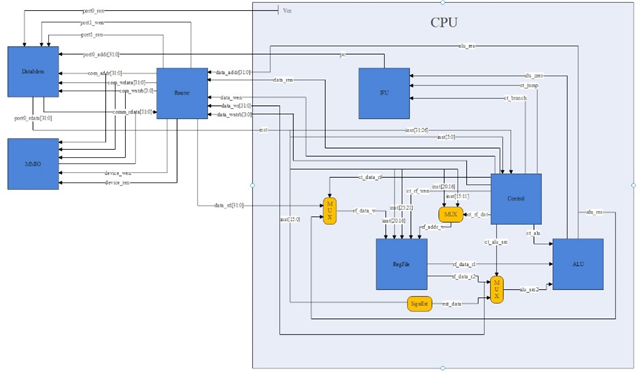
\includegraphics[width=\textwidth]{figure/top}
        \caption{顶层数据通路}
        \label{fig:1}
    \end{figure}

    \subsection{扩展指令后的控制信号表}
    参考示例:
% Table generated by Excel2LaTeX from sheet 'Sheet1'
    \begin{table*}
        \centering
        \caption{控制信号表}
        \begin{tabular}{@{\extracolsep\fill}lll@{\extracolsep\fill}}
            \toprule
            模块                                 & 控制信号         & 作用                                \\
            \midrule
            \multirow{2}[4]{*}{IFU}            & ct\_jump     & 执行跳转指令时变为有效信号                     \\
            \cmidrule{2-3}    \multicolumn{1}{r}{} & ct\_branch   & 执行分支指令时变为有效信号                     \\
            \midrule
            \multirow{2}[4]{*}{DataMem}        & ct\_mem\_wen & 往DataMem写入数据时变为有效信号               \\
            \cmidrule{2-3}    \multicolumn{1}{r}{} & ct\_mmm\_ren & 从DataMem读出数据时变为有效信号               \\
            \midrule
            ALU                                & ct\_alu      & 选择ALU要执行的运算,例如选择执行加法或其他运算         \\
            \midrule
            \multirow{3}[6]{*}{Mux}            & ct\_alu\_src & \multirow{3}[6]{*}{二选一多路选择器的控制信号} \\
            \cmidrule{2-2}    \multicolumn{1}{r}{} & ct\_rf\_dst  & \multicolumn{1}{r}{}              \\
            \cmidrule{2-2}    \multicolumn{1}{r}{} & ct\_data\_rf & \multicolumn{1}{r}{}              \\
            \midrule
            RegFile                            & ct\_rf\_wen  & 往RegFile写入数据数据时变为有效信号             \\
            \bottomrule
        \end{tabular}%
        \label{tab:1}%
    \end{table*}%

    % Table generated by Excel2LaTeX from sheet 'Sheet1'
    \begin{table*}
        \centering
        \caption{控制信号}
        \begin{tabularx}{\linewidth}{@{\extracolsep\fill}llccccc@{\extracolsep\fill}}
            \toprule
            控制                       & 信号名                           & R型  & lw & sw & addiu & bne \\
            \midrule
            \multirow{6}[12]{*}{输入}  & \multirow{6}[12]{*}{ct\_inst} & 0   & 1  & 1  & 0     & 0   \\
            \cmidrule{3-7}           &                               & 0   & 0  & 0  & 0     & 0   \\
            \cmidrule{3-7}           &                               & 0   & 0  & 1  & 1     & 0   \\
            \cmidrule{3-7}           &                               & 0   & 0  & 0  & 0     & 1   \\
            \cmidrule{3-7}           &                               & 0   & 1  & 1  & 0     & 0   \\
            \cmidrule{3-7}           &                               & 0   & 1  & 1  & 1     & 1   \\
            \midrule
            \multirow{10}[20]{*}{输出} & cr\_rf\_dst                   & 1   & 0  & x  & 0     & x   \\
            \cmidrule{2-7}           & cr\_rf\_wen                   & 1   & 1  & 0  & 1     & 0   \\
            \cmidrule{2-7}           & ct\_alu\_src                  & 0   & 1  & 1  & 1     & 0   \\
            \cmidrule{2-7}           & ct\_alu\_op                   & 100 & 0  & 0  & 000   & 001 \\
            \cmidrule{2-7}           & ct\_beq                       & 0   & 0  & 0  & 0     & 0   \\
            \cmidrule{2-7}           & ct\_bne                       & 0   & 0  & 0  & 0     & 1   \\
            \cmidrule{2-7}           & ct\_mem\_ren                  & 0   & 1  & 0  & 0     & 0   \\
            \cmidrule{2-7}           & ct\_mem\_wen                  & 0   & 0  & 1  & 0     & 0   \\
            \cmidrule{2-7}           & ct\_data\_rf                  & 0   & 1  & x  & 0     & x   \\
            \cmidrule{2-7}           & ct\_jump                      & 0   & 0  & 0  & 0     & 0   \\
            \bottomrule
        \end{tabularx}%
        \label{tab:2}%
    \end{table*}%


    \FloatBarrier
    \subsection{扩展指令后的有改动的工程文件代码}

    改动位置用\hl{蓝色字体加粗}显示以示区分,并添加适当注释。


    \begin{lstlisting}[caption = 文件名1.v]
`timescale 1ns / 1ps

module IFU(

);


endmodule
    \end{lstlisting}

    \begin{lstlisting}[caption = 文件名2.v]
module CPU(
input clk,rst
);


endmodule
    \end{lstlisting}

    \FloatBarrier
    \section{仿真文件代码}
    \begin{lstlisting}[caption = 文件名.v]
`timescale 1ns / 1ps

module CPU_tb;




endmodule
    \end{lstlisting}

    \FloatBarrier
    \subsection{CPU运行的程序文件}
    注意,包括\hl{用于测试的汇编代码}和\hl{对应的机器码}

    \begin{lstlisting}[caption = 文件名.asm]
nop // 我们的 IFU 结构决定了第一条是空,没有作用
addiu $8, $0, 1 // t0 是 x0
addiu $9, $0, 1 // t1 是 x1
addiu $10, $0, 10 // t2 号作为 n,设置为 4
addiu $11, $0, 1 // t3 号做为 i
beq $11, $10, 5 // 如果 i 和 n 相等那么往后跳 6 条指令
addu $12, $8, $9 // x2 = x0 + x1 ,t4 是 x2
addiu $8, $9, 0 // x0 = x1
addiu $9, $12, 0 // x1 = x2
addiu $11, $11, 1 // i++
j 5 // 跳转到 beq 这条指令
j 0 // 跳转回初始指令,保证指令能够构成一个大的循环
    \end{lstlisting}
    将其汇编为16进制的机器语言,并写入 \texttt{inst.data} 中,具体如下:

    \begin{lstlisting}[caption = inst.data]
00000000 //nop
24080001 //$8=$0+1
24090001 //$9=$0+1
240a0004 //$10=$0+4
240b0001 //$11=$0+1
116a0005 //if($11==$10)PC=PC+4+5<<2
01096021 //$12=$8+$9
25280000 //$8=$9
25890000 //$9=$12
256b0001 //$11=$11+1
08000005 //j5
08000000 //j0
    \end{lstlisting}

    \section{实验结果与分析}
    \hl{仿真波形图:}

    \hl{仿真波形中与扩展指令相关的关键信号值的分析,及实验结果分析。}

    在vivado中仿真结果如下:
    \begin{figure}[H]
        \centering
        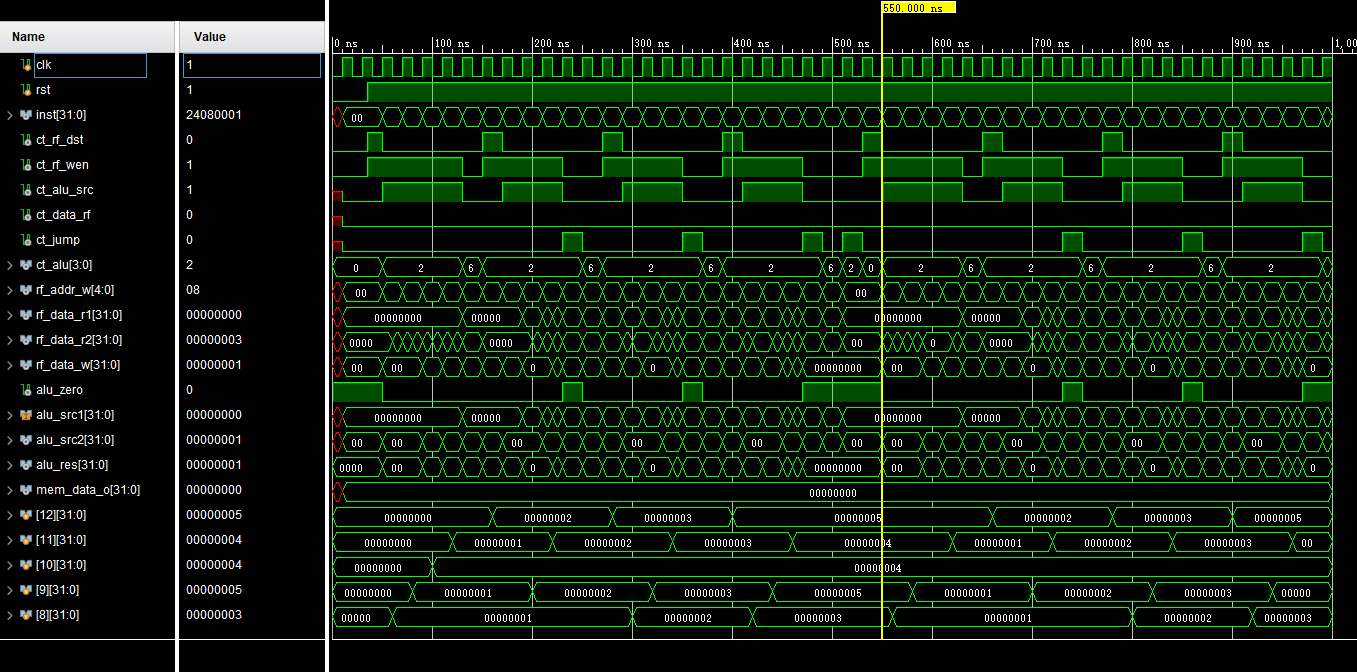
\includegraphics[width=\linewidth]{figure/image2}
        \caption{整体仿真波形图}
    \end{figure}
    首先,对IFU的inst[31:0]进行查看,发现随着始终周期变化时,inst会发生变化,且其中的数据与inst.data中一致,说明IFU指令读取没有问题。

    \begin{figure}[H]
        \centering
        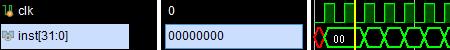
\includegraphics[width=\linewidth]{figure/image3}
        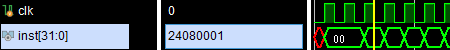
\includegraphics[width=\linewidth]{figure/image4}
        \caption{inst的仿真波形图}
    \end{figure}

    控制器也能够根据之前所写的控制信号表产生相应变化且变化正确,说明控制器没问题。
    \begin{figure}[H]
        \centering
        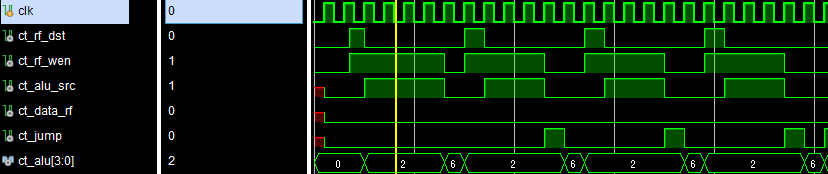
\includegraphics[width=\linewidth]{figure/image5}
        \caption{控制器控制信号的仿真波形图}
    \end{figure}

    对于ALU模块,也能根据不同的指令完成对应的加减法运算。
    \begin{figure}[H]
        \centering
        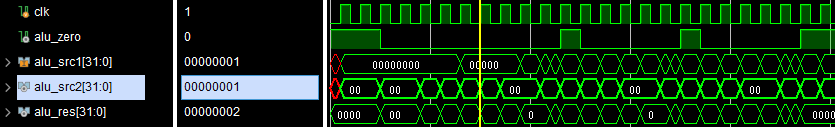
\includegraphics[width=\linewidth]{figure/image6}
        \caption{ALU模块内一些信号的仿真波形图}
    \end{figure}

    寄存器模块同理,也能够根据之前所写的控制信号表产生相应变化且变化正确。
    且上述代码中所用到的8、9、10、11、12号寄存器也可以根据程序的运行过程产生相应变化。
    \begin{figure}[H]
        \centering
        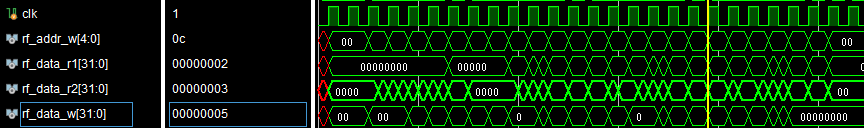
\includegraphics[width=\linewidth]{figure/image7}
        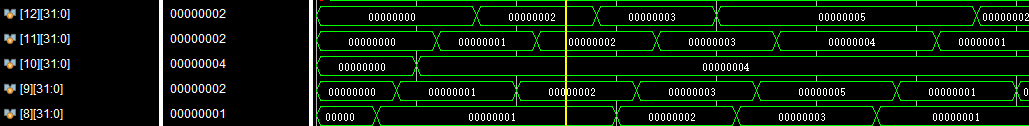
\includegraphics[width=\linewidth]{figure/image8}
        \caption{寄存器及相应信号的仿真波形图}
    \end{figure}

    下面具体分析这些指令的执行过程:
    首先发现空语句能够正确执行;
    之后执行一系列addiu指令,用以8、9、10、11号寄存器赋值,观察到赋值正确,addu指令正确执行;

    \begin{figure}[H]
        \centering
        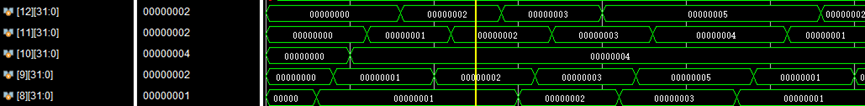
\includegraphics[width=\linewidth]{figure/image9}
        \caption{addiu指令执行分析}
    \end{figure}

    再之后进行beq指令,src1与src2相减判断不为零,不跳转,顺序执行。
    \begin{figure}[H]
        \centering
        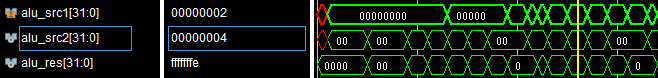
\includegraphics[width=\linewidth]{figure/image10}
        \caption{beq指令执行分析}
    \end{figure}

    之后进行利用addiu进行一系列操作、计算结果正确。
    然后执行j指令进行跳转,跳转后结果正确
    \begin{figure}[H]
        \centering
        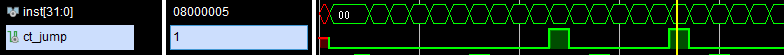
\includegraphics[width=\linewidth]{figure/image11}
        \caption{j指令执行分析}
    \end{figure}

    后续分析同理,不再赘述。最终可以看到满足beq跳转条件,跳出斐波那契计算过程,之后执行j0指令回到初始的第一条指令。
    以上测试说明了CPU各个基本模块能够按照设计正常工作,以及基本指令的执行能够正常完成。




\end{document}